% !Mode:: "TeX:UTF-8"
% !TEX program  = xelatex
\documentclass[withoutpreface,bwprint]{cumcmthesis}
\usepackage{gbt7714}
\bibliographystyle{gbt7714-numerical}



%%%%%%%%%%%%%%%%%%%Tex中常用、好用的宏包%%%%%%%%%%%%%%%%%%%%%%%%%%%%%

%\usepackage{top=25mm,bottom=25mm,left=25mm,right=25mm}{geometry}%调整页边距宏包
	
\usepackage{array} %公式大括号
\usepackage{booktabs}

\usepackage{fancyhdr} % 设置页眉、页脚
\pagestyle{fancy}
\cfoot{第 \thepage 页}
%\pagestyle{empty}
\usepackage{listings} %插入代码块 宏包

\usepackage{xcolor} %背景颜色填充 宏包

\usepackage{graphicx} %图片操作 宏包

\usepackage{pdfpages} %插入pdf文件 宏包



\usepackage{algorithm} %插入伪代码宏包
\usepackage{algorithmic} %插入伪代码宏包
%\usepackage{algorithm2e} %插入伪代码宏包

\usepackage{ulem} %下划线样式宏包


\usepackage{mathrsfs} %花体字母
 

\usepackage{amsopn} %自定义预置符号函数
\DeclareMathOperator{\Sign}{\mathbb{P}\mathbb{e}\mathbb{i}\mathcal{t}\mathcal{s}\mathcal{a}\mathcal{n}}

\DeclareMathOperator{\tx}{\mathbb{X}} 

%%%%%%%%%%%%%%%%%%%Tex中常用、好用的宏包%%%%%%%%%%%%%%%%%%%%%%%%%%%%%

\title{Hello Styles}
\tihao{A}            % 题号
\baominghao{114514}    % 报名号
\schoolname{重庆邮电大学}
\membera{Peitsan}
\memberb{ShiyanGG}
\memberc{LihaoGG}
\supervisor{Boss Shen}
\yearinput{2022}     % 年
\monthinput{09}      % 月
\dayinput{13}        % 日

\begin{document}
	\maketitle
	\begin{abstract}
		。摘要的具体内容。摘要的具体内容。摘要的具体内容。摘要的具体内容。
		\keywords{关键词1\quad  关键词2\quad   关键词3}
	\end{abstract}
	
	
\newpage
%	\geometry{top=25mm,bottom=25mm,left=25mm,right=25mm}
	\tableofcontents
\newpage

\section{Tex中常用、好用的宏包}	

	\noindent 1.listings
	%设置代码框样式
	\lstset{
		columns=fixed,       
		numbers=left,                                        % 在左侧显示行号
		numberstyle=\tiny\color{gray},                       % 设定行号格式
		frame=shadowbox,                                          % 不显示背景边框
		backgroundcolor=\color[RGB]{255,255,255}, 
		keywordstyle=\color[RGB]{40,40,255},                 % 设定关键字颜色
		numberstyle=\footnotesize\color{darkgray},           
		commentstyle=\it\color[RGB]{0,96,96},                % 设置代码注释的格式
		stringstyle=\rmfamily\slshape\color[RGB]{128,0,0},   % 设置字符串格式
		showstringspaces=false,                              % 不显示字符串中的空格
		language=c++,                                        % 设置语言
	}
	
	
	\begin{lstlisting}[title=code1,frame=shadowbox,language=c++]
				#include <iostream>
				using namespace std;
				
				int main()
				{
					cout<<"hello"<<endl;
					return 0;
				}
	\end{lstlisting}

		\begin{lstlisting}[title=code1,frame=shadowbox,language=matlab]
		%% 第二问求解
		%% 三发射机代码
		%已知FY_00和FY_01发射机之间的夹角为a1
		%三架发射机其中一架未知编号求解代码
		%因算法特性会有多种loss值较小的情况无法精准定位,故三架发射机不可行
		% clc;clear
		% load location.mat
		% disp('假设不知道编码的飞机为FY_X')
		% angle=input('请依次输入接收机得到的信息<FY_00,FY_01> <FY_00,FY_X> <FY_01_X>(例如[20 20 40])');
		% loss_list=[];%存储每个循环总损失
		% 
		% for i=2:9
		%     fly_item=[1 i];
		%     out=main_fun(angle,fly_item);
		%     loss=loss_fun1(location,out,fly_item);
		%     loss_list=cat(1,loss_list,loss);
		% end
		%     item=find(min(loss_list(:,1))==loss_list(:,1));%最小损失
		%     disp(['未知无人机的标号为' num2str(loss_list(item,2))])
		%     disp(['其损失loss=' num2str(loss_list(item,1))])
		
		%% 四发射机代码
		clc;clear
		load location.mat
		disp('假设不知道编码的飞机为FY_X1,FY_X2')
		angle1=input('请依次输入接收机得到的关于FY_X1的信息<FY_00,FY_01> <FY_00,FY_X1> <FY_01,FY_X1>(例如[20 20 40])');
		angle2=input('请依次输入接收机得到的关于FY_X2的信息<FY_00,FY_01> <FY_00,FY_X2> <FY_01,FY_X2>(例如[20 20 40])');
		loss_list=[];%存储每个循环总损失
		
		for i=2:9
		for j=i+1:9
		if i~=j
		fly_item=[1 i j];
		out1=main_fun(angle1,fly_item(1:2));
		out2=main_fun(angle2,fly_item(1:2:3));
		loss=loss_fun2(location,out1,out2,fly_item);
		loss_list=cat(1,loss_list,loss);
		end
		end
		end
		item=find(min(loss_list(:,1))==loss_list(:,1));%最小损失
		disp(['未知无人机的标号分别为' '  FY_0' num2str(loss_list(item,2)) ', FY_0' num2str(loss_list(item,3))])
		disp(['其损失loss=' num2str(loss_list(item,1))])
		%至此已知全部发射机的编号,此后可用第一问模型进行求解定位
		
	\end{lstlisting}


	\lstinputlisting[title=第一问的C++代码,language=c++,frame=none]{code/codetest.cpp}
	
	\lstinputlisting[title=第一问的MATLAB代码,language=matlab,frame=none]{code/code\_1\_2.m}
	
	
	\noindent 2.xcolor
	
	
	\textcolor{y}{这是一段黄色的文字}
	%设置文字颜色的宏包,使用自定义和预定义的颜色
	%改变文字的背景色
	\colorbox{Purple}{修改背景颜色为紫色}
	
	%产生一个红色背景色,蓝色边框的效果
	\fcolorbox{blue}{red}{文字加上蓝色边框、红色背景}
	
	\noindent 3.graphics插入图片
	
	
\includegraphics[height=2cm]{figures/sample.png}
	
	\noindent 4.pdfpages插入pdf 可以指定页码
	
	
\includepdf[pages=1]{figures/cat.pdf}
	
	\newpage
	
	\noindent 5.algorithm|algorithmic 编写伪代码
	
\begin{algorithm}[htbp!]
	\caption{PARTITION$(A,p,r)$}%算法标题
	\begin{algorithmic}[1]%一行一个标行号
		\STATE $i=p$
		\FOR{$j=p$ to $r$} % for(int j=p ; j<=r; j++)
			\IF{$A[j]<=0$}
				\STATE $swap(A[i],A[j])$
				\STATE $i=i+1$
			\ENDIF
		\ENDFOR
	\end{algorithmic}
\end{algorithm}


%\newtheorem{definition}{\mcm@cap@definition}
%\newtheorem{theorem}{\mcm@cap@theorem}
%\newtheorem{lemma}{\mcm@cap@lemma}
%\newtheorem{corollary}{\mcm@cap@corollary}
%\newtheorem{assumption}{\mcm@cap@assumption}
%\newtheorem{conjecture}{\mcm@cap@conjecture}
%\newtheorem{axiom}{\mcm@cap@axiom}
%\newtheorem{principle}{\mcm@cap@principle}
%\newtheorem{problem}{\mcm@cap@problem}
%\newtheorem{example}{\mcm@cap@example}
%\newtheorem{proof}{\mcm@cap@proof}
%\newtheorem{solution}{\mcm@cap@solution}
	
	\noindent 6.amsmath|amssymb|amsfonts 特殊符号
	
	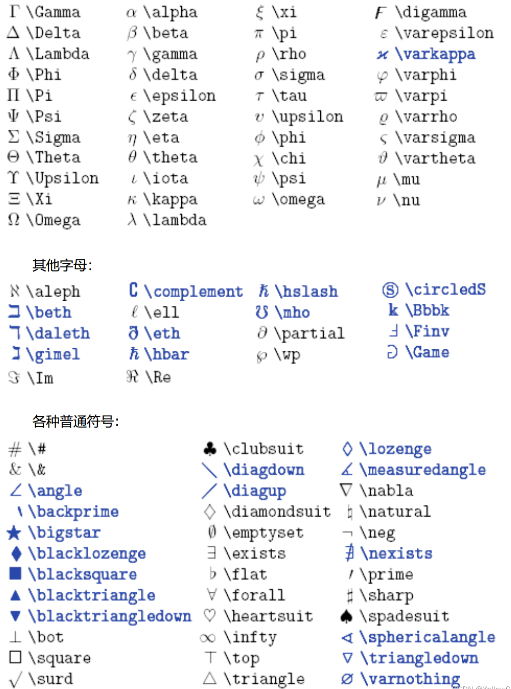
\includegraphics[width=12cm]{figures/signal.png}
	
	\newpage
	\noindent 7.ulem 下划线格式拓展
	
	\underline{内置下划线命令}
	
	This is \emph{emph}. %强调
	
	This is \uline{uline} %单下划线
	
	This is \uuline{uuline} %双下划线
	
	This is \uwave{uwave} %波浪线
	
	This is \sout{sout} %正中删除线
	
	This is \dotuline{dotuline} %点线
	
	This is \dashuline{dashuline} %虚线
	
	This is \xout{xout}\par %斜删除线
	
	\noindent 8.mathrsfs 花体字母
	
	$\mathbb{D}$
	
	$\mathcal{X}$ 
	
	$\mathscr{LBC}$  $\mathscr{A}$  $\mathscr{M}$
	
	\noindent 9.amsopn 自定义符号函数
	
	%\DeclareMath0perator{\新函数命令}{新函数名}
	
	可以在导言区自定义类似 \verb*|\sim| 和 \verb*|\lim| 等新的算符 或函数;也可以在正文中用它提供的命令\verb*|\operatorname{函数名}|,自定义临时使用的函数。举例说明:
	
	$\tx$
	
	$\Sign$
	
	\newpage
	\bibliography{bib/cite.bib}
	\newpage
	
	\noindent 10.页边距、页眉页脚
	
	页眉页脚通常出现页码、姓名学号、标题等等。在上一节中,提及到页码在右上角,有时候又在中间,那如何做到统一规范,需要使用如下指令以及包。这里如果使用了此包,则对应的pagestyle要设置为fancy才能单独修改每一部分。
	
		\lhead{2021212961}%页眉左边
		\chead{第一章}%页眉中间
		\rhead{题目编号 A题}%页眉右边
		\lfoot{xxxx}%页脚左边
		\cfoot{第\thepage 页}%页脚中间
		\rfoot{yyy}%页脚右边
	
	这里要说明,对于使用\\maketitle指令所在的页面,是不会出现页眉页脚的。
	
	\newpage %这里表示A页
	\pagestyle{headings}%表示A页中不要页脚
	AAAAAA
	\newpage %这里表示B页
	\pagestyle{plain}%表示B页中不要页脚
	BBBBBB
	\newpage%这里表示C页
	\pagestyle{empty}%表示C页中不出现页眉页脚
	
	
	11.列举标题
		
		\quad \begin{itemize}
			\item[1.] 第一步
			\item[2.] 第二步
			\item[3.] 第三步
			\item[4.] 第四步
			\item[5.] 第五步
		\end{itemize}
	
	
\assumption{这是假设}

\assumption{这是假设}

\assumption{这是假设}
	
\definition{定义}
\theore{定理}
\corollary{引理}

\conjectur{猜想}
\definition{定义}
\definition{定义}
\definition{定义}

%	\newcommand*{\mcm@cap@theorem}{定理}
%	\newcommand*{\mcm@cap@lemma}{引理}
%	\newcommand*{\mcm@cap@corollary}{推论}
%	\newcommand*{\mcm@cap@assumption}{假设}
%	\newcommand*{\mcm@cap@conjecture}{猜想}
%	\newcommand*{\mcm@cap@axiom}{公理}
%	\newcommand*{\mcm@cap@principle}{定律}
%	\newcommand*{\mcm@cap@problem}{问题}
%	\newcommand*{\mcm@cap@example}{例}
%	\newcommand*{\mcm@cap@proof}{证明}
%	\newcommand*{\mcm@cap@solution}{解}
	
	
	
一. -> A
	
二. -> B
	
%	 \renewcommand\appendix{\par
%	 \setcounter{section}{0}%
%	 \setcounter{subsection}{0}%
%	 \gdef\thesection{\appendixname\@Alph\c@section}}
	\appendix 
%		\renewcommand{\appendixname}{Appendix ~\Alph{section}}
		
			\section{附表1——XXXXXX}
			
			\section{附表2——XXXXXX}
			
			\section{附表3——XXXXXX}
	
\end{document}
